

\chapter[MD simulations of PgaB-glucosamine binding]{Molecular Dynamics simulations of PgaB and monosaccharides of N-acetyl-glucosamine}

\emph{Reference}: Part of this work is published in ``PgaB Contains a Carbohydrate Binding Domain Required for Modification and Export of Poly-$\beta$-1,6-N-acetyl-D-glucosamine"
\\
\\
\emph{Contributions}:
Grace Li conducted the MD simulation part of the research and wrote the section. Dustin Little conducted and interpreted the experimental results. Chris Ing parameterized the partial charges for glucosamine. R\'{e}gis Pom\`{e}s, Lynne Howell, Mark Nitz provided editorial input and guidance.

\newpage

\section{Summary}

\section{Introduction}


PgaB is a protein required for the partial de-N-acetylation of poly-$\beta$-1,6-$N$-acetylglucosamine (PNAG) into dPNAG, the functionally-relevant form of the exopolysaccharide essential for biofilm formation in a variety of pathogenic bacteria. \cite{Little:2012dp} The crystal structure of PgaB was recently solved in the laboratory of Dr. Lynne Howell.\cite{Little:2012dp} Structural and functional characterization have shown that PgaB is composed of two domains, an N-terminal domain de-N-acetylase, and a C-terminal domain with structural similarity to glycoside hydrolases.\cite{Little:2012dp}

Although it is known that PgaB functions by binding to PNAG, the molecular basis of the mechanism of export of PNAG by PgaB is currently not determined.  Moreover, the binding mode and the length of its substrate polymer are not known.
Efforts to crystallize PgaB with oligosaccharides of varying lengths have been impeded by the weak binding of short sugar polymers (eg. di- and tri-saccharides), and the insolubility of long sugar polymer chains (eg. those longer than a hexamer). However, molecular dynamics (MD) simulations are not impeded by these challenges and are well-suited for characterizing carbohydrate-protein interactions.\cite{Fadda:2010p5889}

In this study, we perform atomistic MD simulations of PgaB with the monosaccharide components of the functionally-relevant polymer dPNAG, $\beta$-N-acetyl-glucosamine (GlcNAc) and protonated $\beta$-glucosamine (GlcNH$_{3}^{+}$), to examine the putative polymeric binding site and binding mode.  The weak binding affinity of these monosaccharides allows us to use a fragment-based methodology to probe for carbohydrate binding sites.  This method has been employed successfully in our previous studies to examine the binding mechanism of inositol, a carbohydrate-like amyloid inhibitor, with amyloidogenic peptides and their aggregates.\cite{Li:2012bx}


\section{Material and Methods}
A chimeric PgaB structure with the loop spanning residues 613 to 619 in the N-terminal domain modelled into the truncated crystal structure, was used in our simulations. The initial crystal structure has Ni$^{2+}$ bound at its enzymatic active site. Ni$^{2+}$ is octahedrally coordinated with surrounding residues and ligands.  The acetate ion bound to Ni$^{2+}$ near the active site, an artifact of crystallization, was removed in the simulation. Crystal waters were removed from the initial PDB structure. Histidine protonation states were assigned based on predicted pKa values using the web software PROPKA,\cite{Bas:2008ul,Olsson:2011vi,Sondergaard:2011ug} and histidine hydrogen-bonding geometries in the initial crystal structure.

Protein and ions were modelled using the AMBER99 force field.\cite{Cornell:1995td} Parameters for Ni$^{2+}$ were approximated using those of the magnesium ion (Mg$^{2+}$). After assigning protonation states of histidines, the net charge of the protein was -10e. The final simulation system comprised of 11 sodium (Na$^{+}$) counterions, and 45 molecules of free monosaccharride molecules (either GlcNAc or \glucosamine) at an effective concentration of 100 mM (Figure~\ref{fig:nag}). 19533 and 19991 water molecules were present in the GlcNAc and \glucosamine\ simulations, respectively. The initial volume of the simulation box is 713.6 nm$^{3}$.  To mimic experimental conditions, 100 mM of salt was added to the aqueous solution simulation systems containing \glucosamine.

The structure of GlcNAc was generated using the web-based Glycam Biomolecule Builder.\cite{Woods:glycambuilder} The GLYCAM06 force field for carbohydrates\cite{Kirschner:2008ii} was used to model both GlcNAc and \glucosamine. A PDB of \glucosamine\ was obtained from the ZINC database.\cite{Irwin:2005kx} Energy minimization was performed using the software GAUSSIAN-09.\cite{g09} The minimized \glucosamine\ structure was consistent with the GLYCAM force field, and new RESP-derived partial atomic charges were computed for \glucosamine\ (a net charge of +1e) by fitting to a single HF/6-31G* molecular electrostatic potential (MEP) with a restraint weight of 0.01. MEPs were computed using the CHELPG methodology\cite{Breneman:1990ue} with the R.E.D. III software package.\cite{Dupradeau:2010bb} The partial charges were assigned so that the HCNH$_{3}$ group summed to a net charge of +1.164e, and the rest of the molecule summed to a net charge of -0.164e. Aliphatic hydrogen atoms were fitted with a zero partial charge for compatibility with GLYCAM06.


The TIP3P water model was used to represent the solvent. Version 4.5.5 of the GROMACS software package\cite{Pronk:2013ef,Hess:2008p5353} was used to perform unrestrained all-atom MD simulations with the stochastic dynamics algorithm using an integration timestep of 2 femtoseconds.

Electrostatic interactions were calculated using Particle Mesh Ewald (PME) summation with a grid size of 0.12 nm and a Coulombic real-space cutoff of 1.1 nm. The Lennard-Jone potential was computed up to 1.2 nm using the GROMACS twin-range cutoff function with a short-range cut-off of 1.1 nm. Covalent bonds involving hydrogens were constrained using the LINCS algorithm. The simulation system was first subjected to energy minimization followed by a 1 ns equilibration in the NVT ensemble using Berendsen temperature coupling at 300 K with a coupling constant of 2.0.

A second equilibration was performed for 1 ns in the NpT ensemble with isotropic pressure coupling. Temperature and pressure for equilibration were controlled at 300 K and at 1 atm, respectively, using Berendsen thermostat and pressure coupling schemes. Production simulations were performed using the stochastic dynamics (sd) integrator and the Parrinello-Rahman barostat for pressure coupling.

For each of GlcNAc and \glucosamine, 13 independent MD simulations at 130 ns per replica were performed, respectively, yielding a total of 3.38 $\mu$s of sampling time.

\subsection*{Analysis Protocol}
To compute spatial binding probability densities of GlcNAc and \glucosamine, frames from our simulations were first fitted via RMSD alignment of the protein backbone atoms to an energy minimized and MD-equilibrated crystal structure. The density map corresponds to the fractional atomic occupancy of GlcNAc or \glucosamine molecules binned using a grid with 1 \angstrom\ resolution.  The density map for each of GlcNAc and \glucosamine\ was computed using $\sim$165,000 time frames. The Visual Molecular Dynamics (VMD) software package\cite{Humphrey:1996to} was used to calculate and graphically render the densities depicted in Figures~\ref{fig:sdf}, \ref{fig:groove}, and \ref{fig:salt_density_distribution}.

\section{Results and Discussion}


\subsection{Comparisons of the binding modes of GlcNAc and \glucosamine}

The spatial binding probability density of GlcNAc, depicted in Figure~\ref{fig:sdf}, suggests that binding sites for GlcNAc are predominantly located in proximity to the active site (in the N-terminal domain), consistent with the function of PgaB as a PNAG de-acetylase. In particular, the densities in the inter-domain crevice beneath the loop spanning residue numbers 309 to 314 suggest that this region may be involved in substrate binding.  This result corroborates the hypothesis that the binding of PNAG to PgaB may initiate in this region, prior to binding at the active site.\cite{Little:2012dp} 




By contrast, the spatial distribution of \glucosamine\ molecules depicted in Figure~\ref{fig:sdf} indicates that they preferentially bind to the C-terminal domain, with a significant density in the groove heavily lined with acidic and aromatic residues (Figure~\ref{fig:groove}).
Notably, consistent with the crystal structure of the C-terminal domain of PgaB (PgaB-CT) with bound \glucosamine, our simulation results indicate that both GlcNAc and \glucosamine\ possess binding sites at Trp613 and Trp552  (Figure~\ref{fig:groove}), which are conserved residues located in this groove.\cite{Little:2012dp}
In support of this result, our previous study has shown that PgaB-CT is structurally similar to glycoside hydrolases,\cite{Little:2012dp} where the active site for these enzymes is also located in analogous grooves with a similar geometry. 

Furthermore, our results indicate that the entire length of the groove can bind \glucosamine\ molecules, suggesting that this groove is likely to accommodate a linear polymer of \glucosamine\ (Figure~\ref{fig:groove}). Accordingly, in our simulations, \glucosamine\ molecules were observed to bind in this groove by forming linear hydrogen-bonded chains (Figure~\ref{fig:directionality}).  Taken together,  our results suggest that this C-terminal groove of PgaB is a binding site for the de-acetylated PNAG (dPNAG).   In contrast to the spatial distributions of GlcNAc and \glucosamine, salt ions do not significantly bind the protein  (Figure~\ref{fig:salt_density_distribution}). 

Together, the morphology of the overall binding density of both GlcNAc and \glucosamine\ paints a molecular picture of the putative binding mechanism and export of PNAG. As PNAG is being shuttled through PgaB on to the next protein in the system, it initially binds at the cleft between the N- and C-terminal domains to reach the active site in order to undergo de-N-acetylation.  Our simulations suggest that as the polymer is de-acetylated, the binding affinity of the resulting dPNAG to the C-terminal domain is increased. This hypothesis is currently being validated experimentally. We propose that PgaB-CT facilitates the export of  the substrate by favorably binding its de-acetylated region.  






This study demonstrates the utility of large-scale MD simulations in predicting carbohydrate-protein binding modes when combined with a force field that can reproduce sugar-protein interactions with relative accuracy (for example, GLYCAM\cite{Kirschner:2008ii}). Force fields for molecular simulations of carbohydrates have been recently reviewed here.\cite{Fadda:2010p5889}  Furthermore, we demonstrated the utility of computing spatial probability binding densities using monosaccharides to map carbohydrate binding sites. A recent study suggests that by building 3D density binding maps of carbohydrates and using this data with additional computational algorithms can increase the accuracy of identifying putative carbohydrate binding sites.\cite{Tsai:2012bj} As part of future work, it may be interesting to employ a similar approach to investigate the binding of oligosaccharides to PgaB.  





\section{Acknowledgements}
This work was done in collaboration with Dustin Little, Dr. Lynne Howell and Dr. Mark Nitz.

\section{Figures}

\begin{figure}[htbp]
\centering
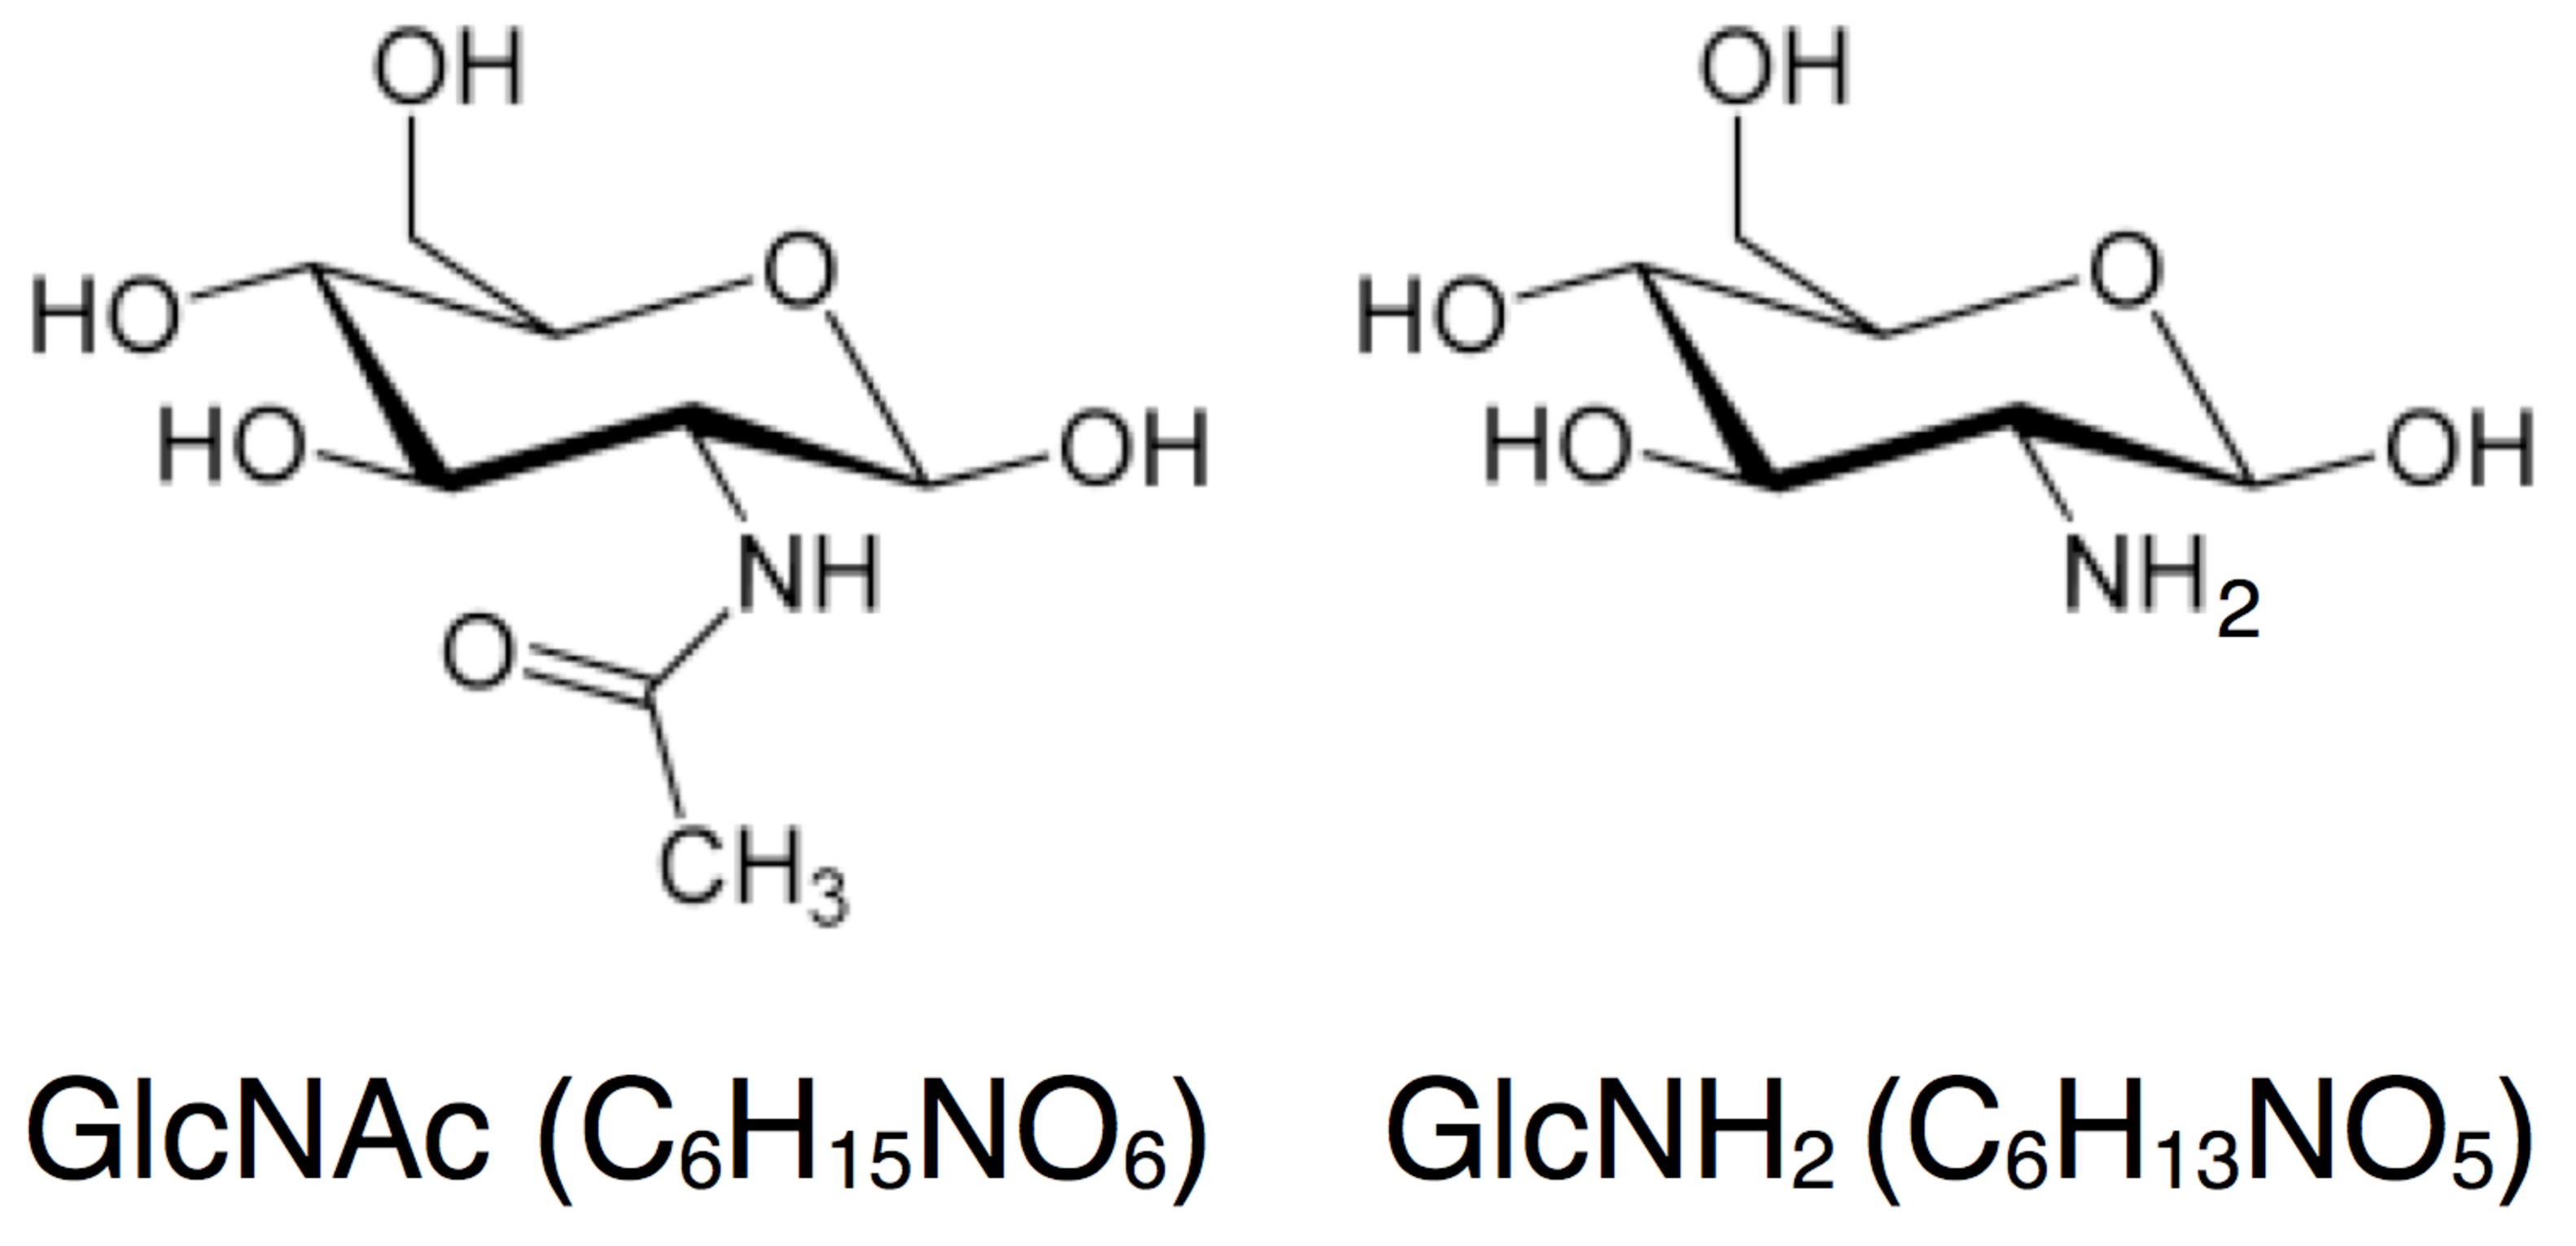
\includegraphics[width=4in]{figures/results4/sugar_structures.pdf}
\caption[Molecular structures of GlcNAc and GlcNH$_2$]{Molecular structures of $\beta$-N-acetyl-glucosamine (GlcNAc) and $\beta$-glucosamine (GlcNH$_2$).}
\label{fig:nag}
\end{figure}



\begin{figure}[htbp]
\centering
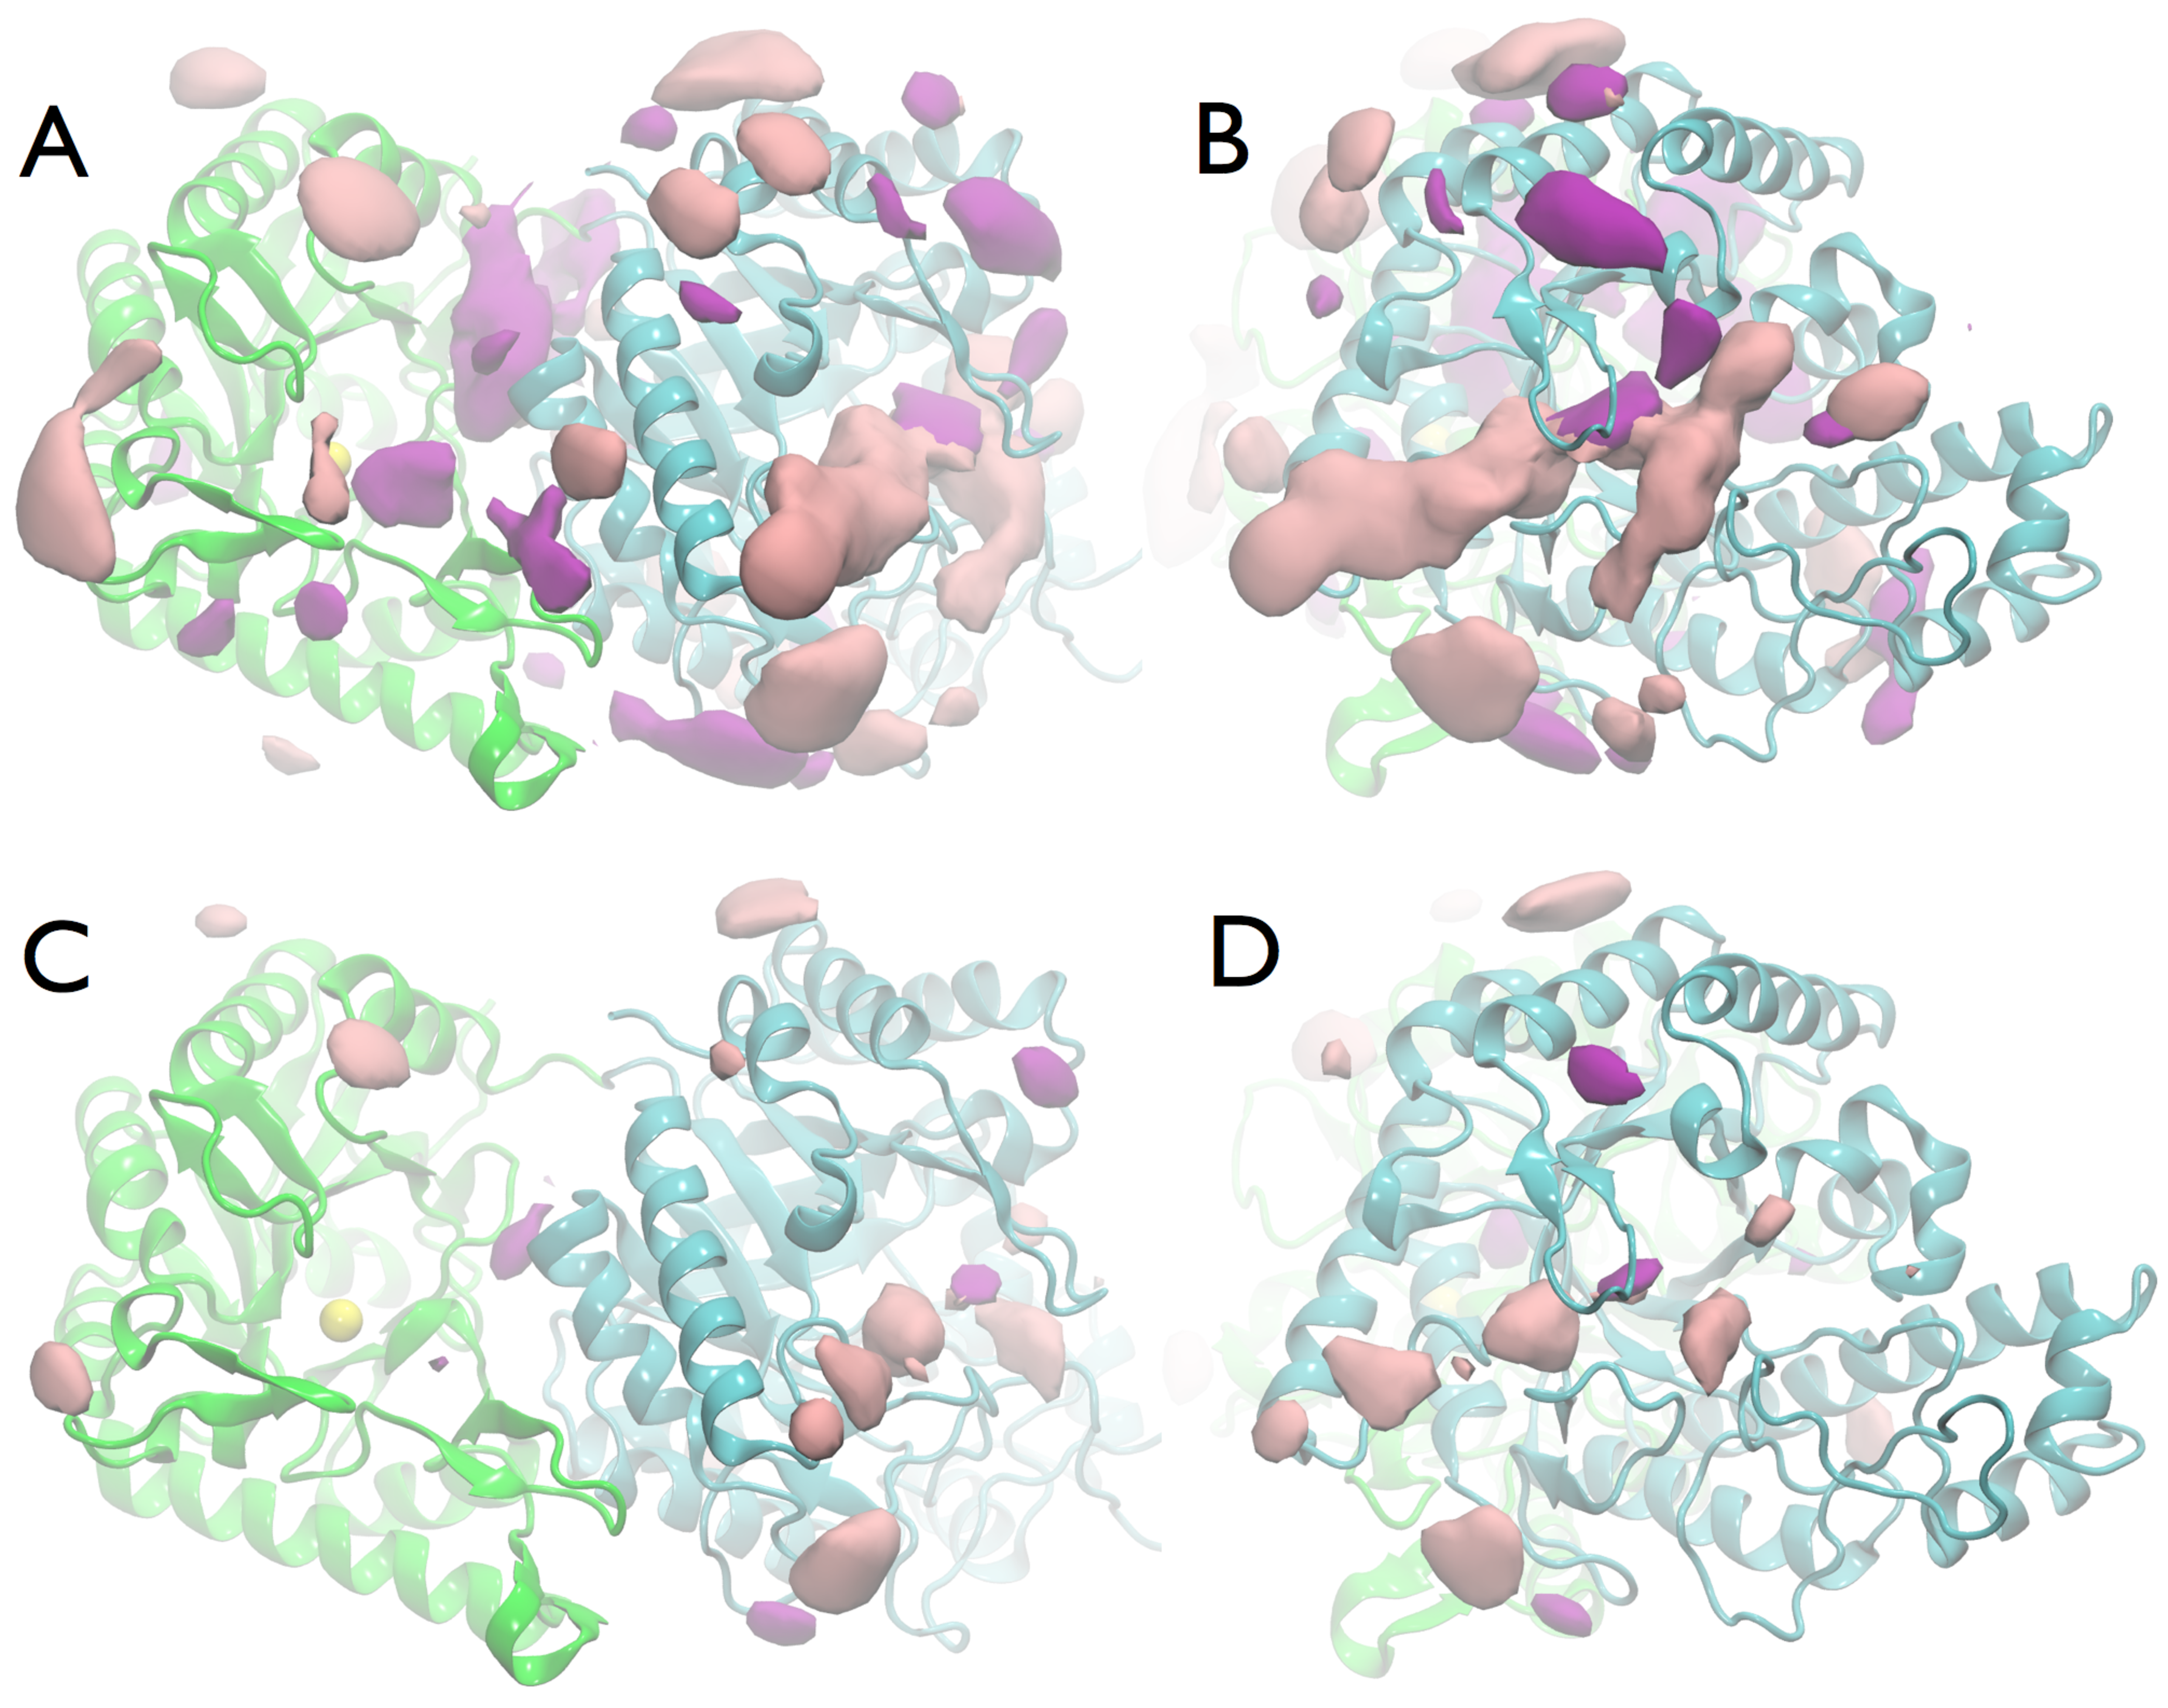
\includegraphics[width=6.25in]{figures/results4/glcnac_glucosamine_merged_sdf.pdf}
\caption[Spatial probability densities of bound GlcNAc (purple) and \glucosamine]{Spatial probability densities of bound GlcNAc (purple) and \glucosamine\ (pink).  Binding densities overlapped with a cartoon representation of the energy minimized crystal structure of PgaB.  The protein is shown facing the active site in (A) and (C), and shown facing the C-terminal domain in (B) and (D). In each view, binding densities are depicted at occupancies of 0.15 in (A)-(B), and 0.25 in (C) - (D). In our coloring scheme, residue numbers 43 to 310 and numbers 311 to 667 represent N- (green) and C-terminal (cyan) domains, respectively.}
\label{fig:sdf}
\end{figure}

\begin{figure}[htbp]
\centering
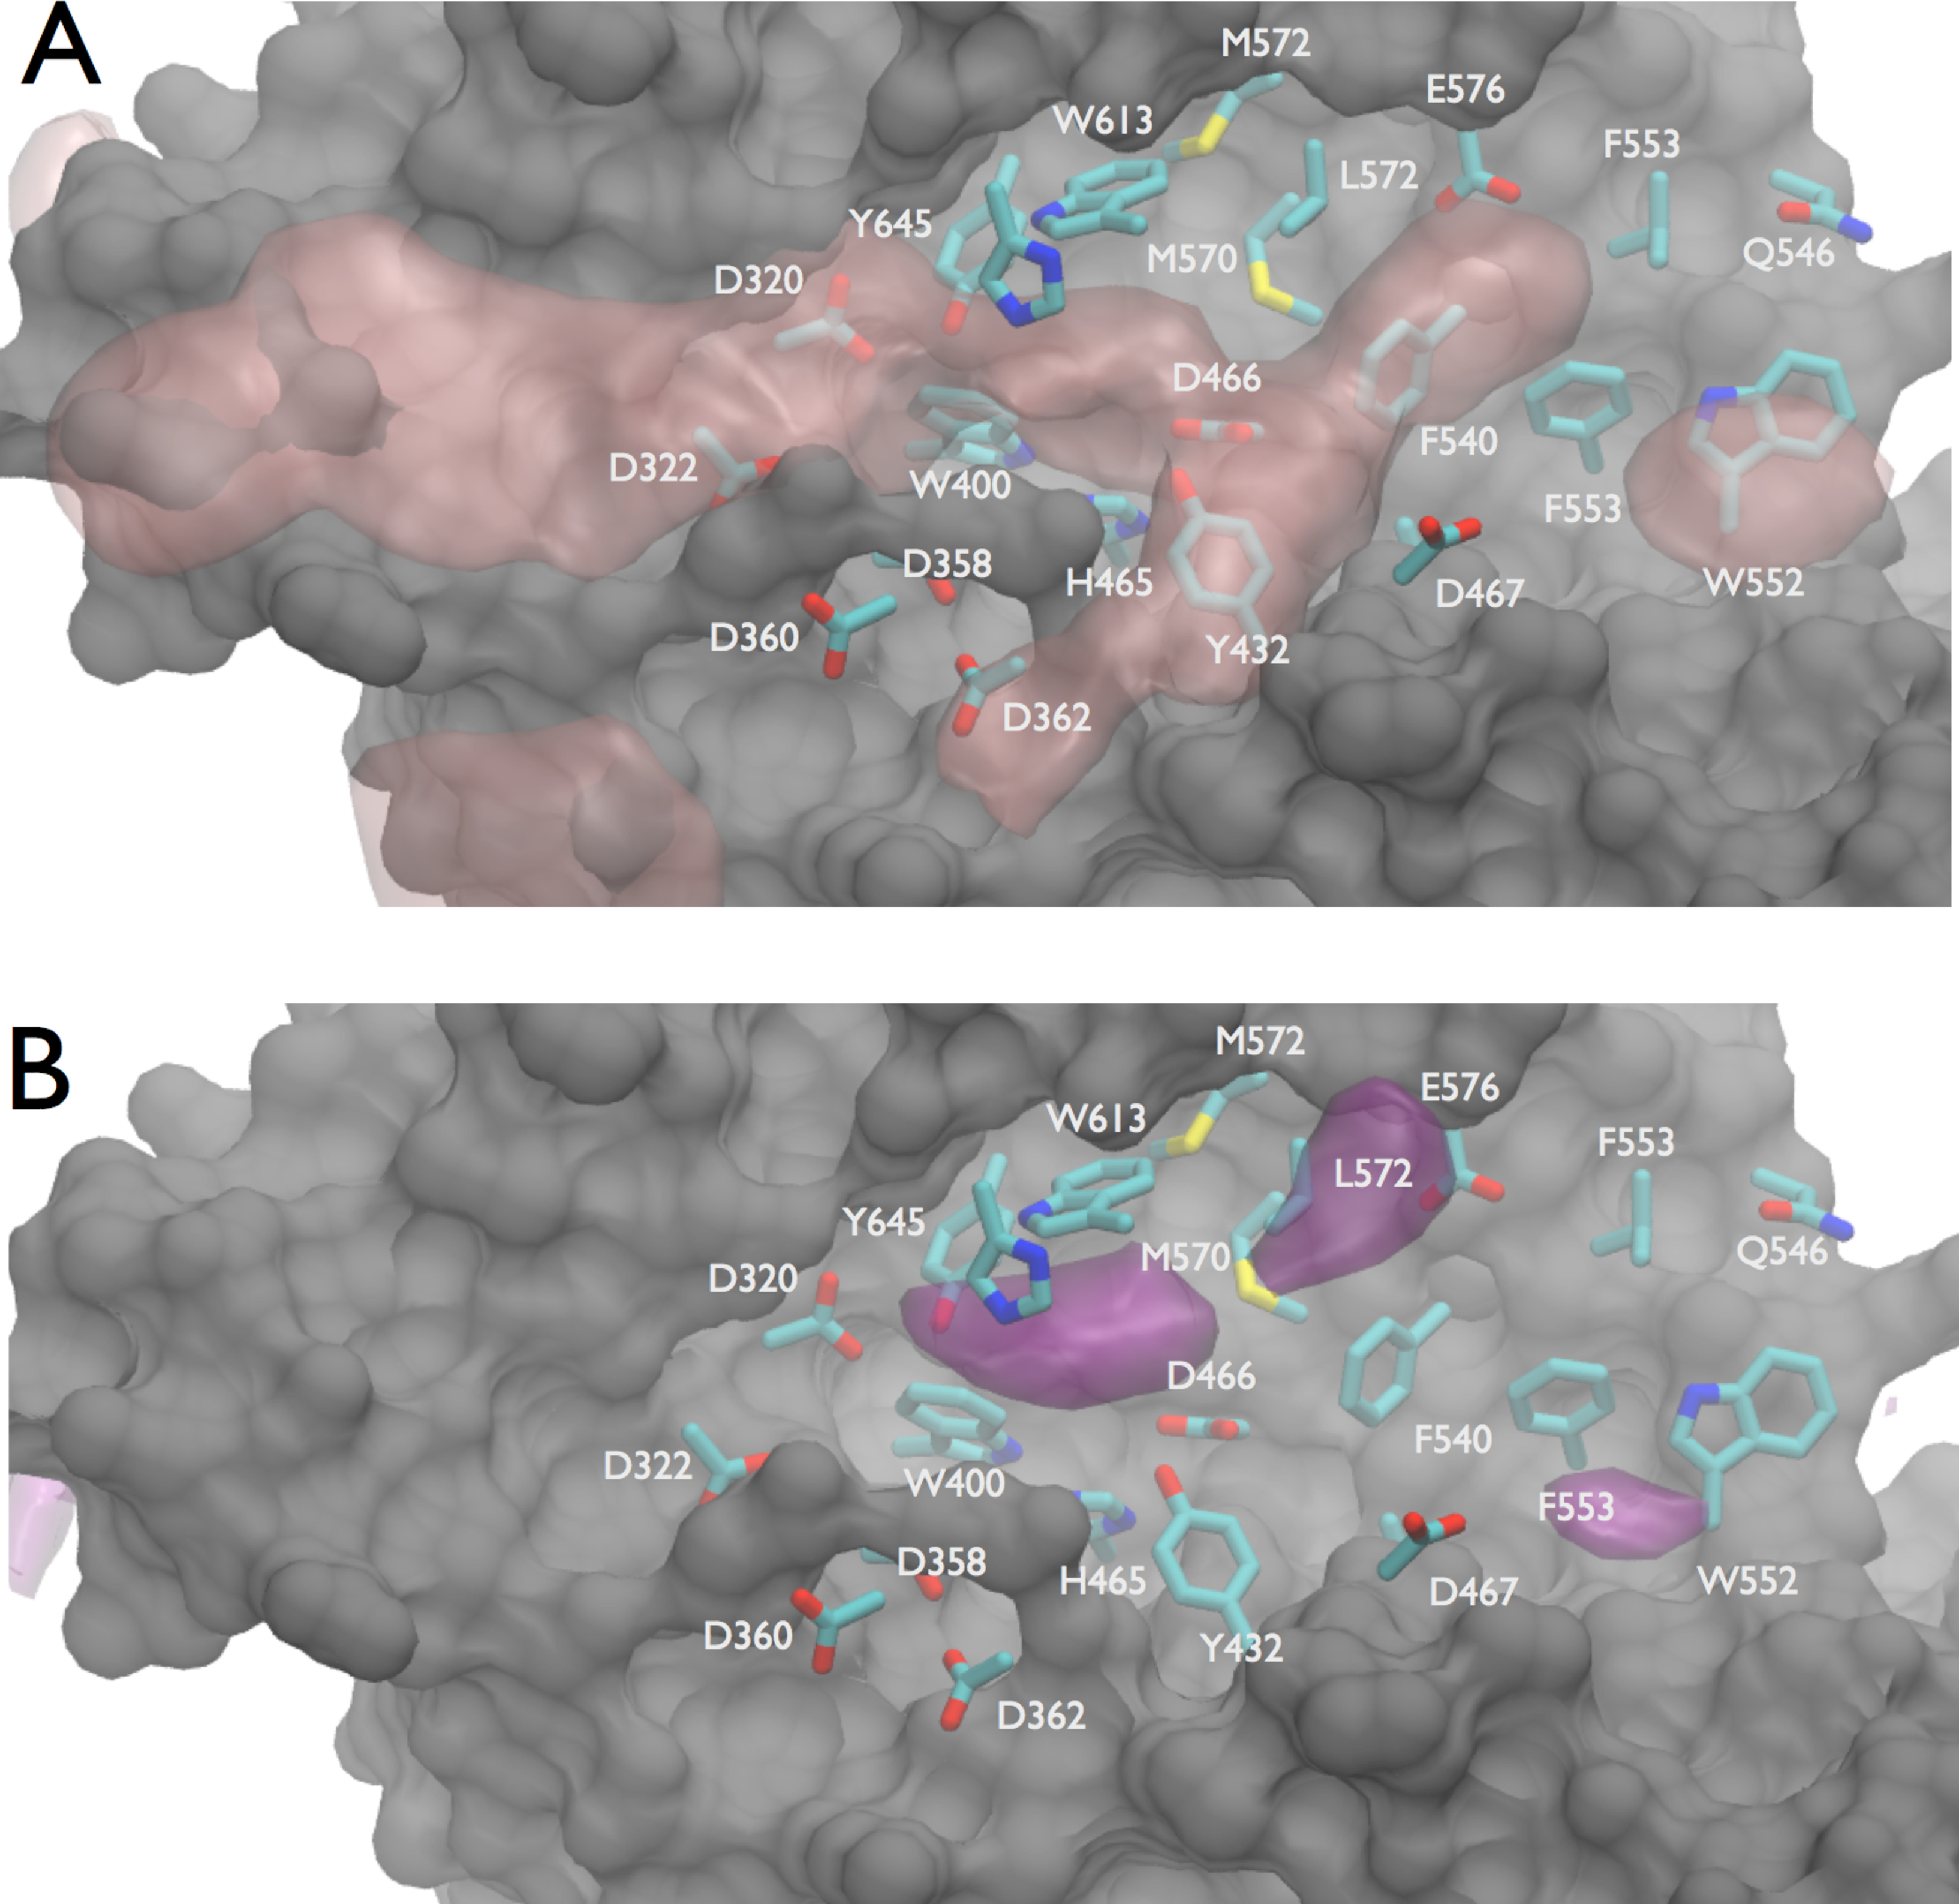
\includegraphics[width=6.25in]{figures/results4/cterm_groove_surf2.pdf}
\caption[Spatial probability densities of GlcNAc and GlcNH3+ in the C-terminal groove]{Spatial probability distribution shown at an occupancy of 0.15 for (A) \glucosamine\ and (B) GlcNAc in the binding groove of the C-terminal domain.  The residues in the groove are shown in stick representations.}
\label{fig:groove}
\end{figure}

\begin{figure}[htbp]
\centering
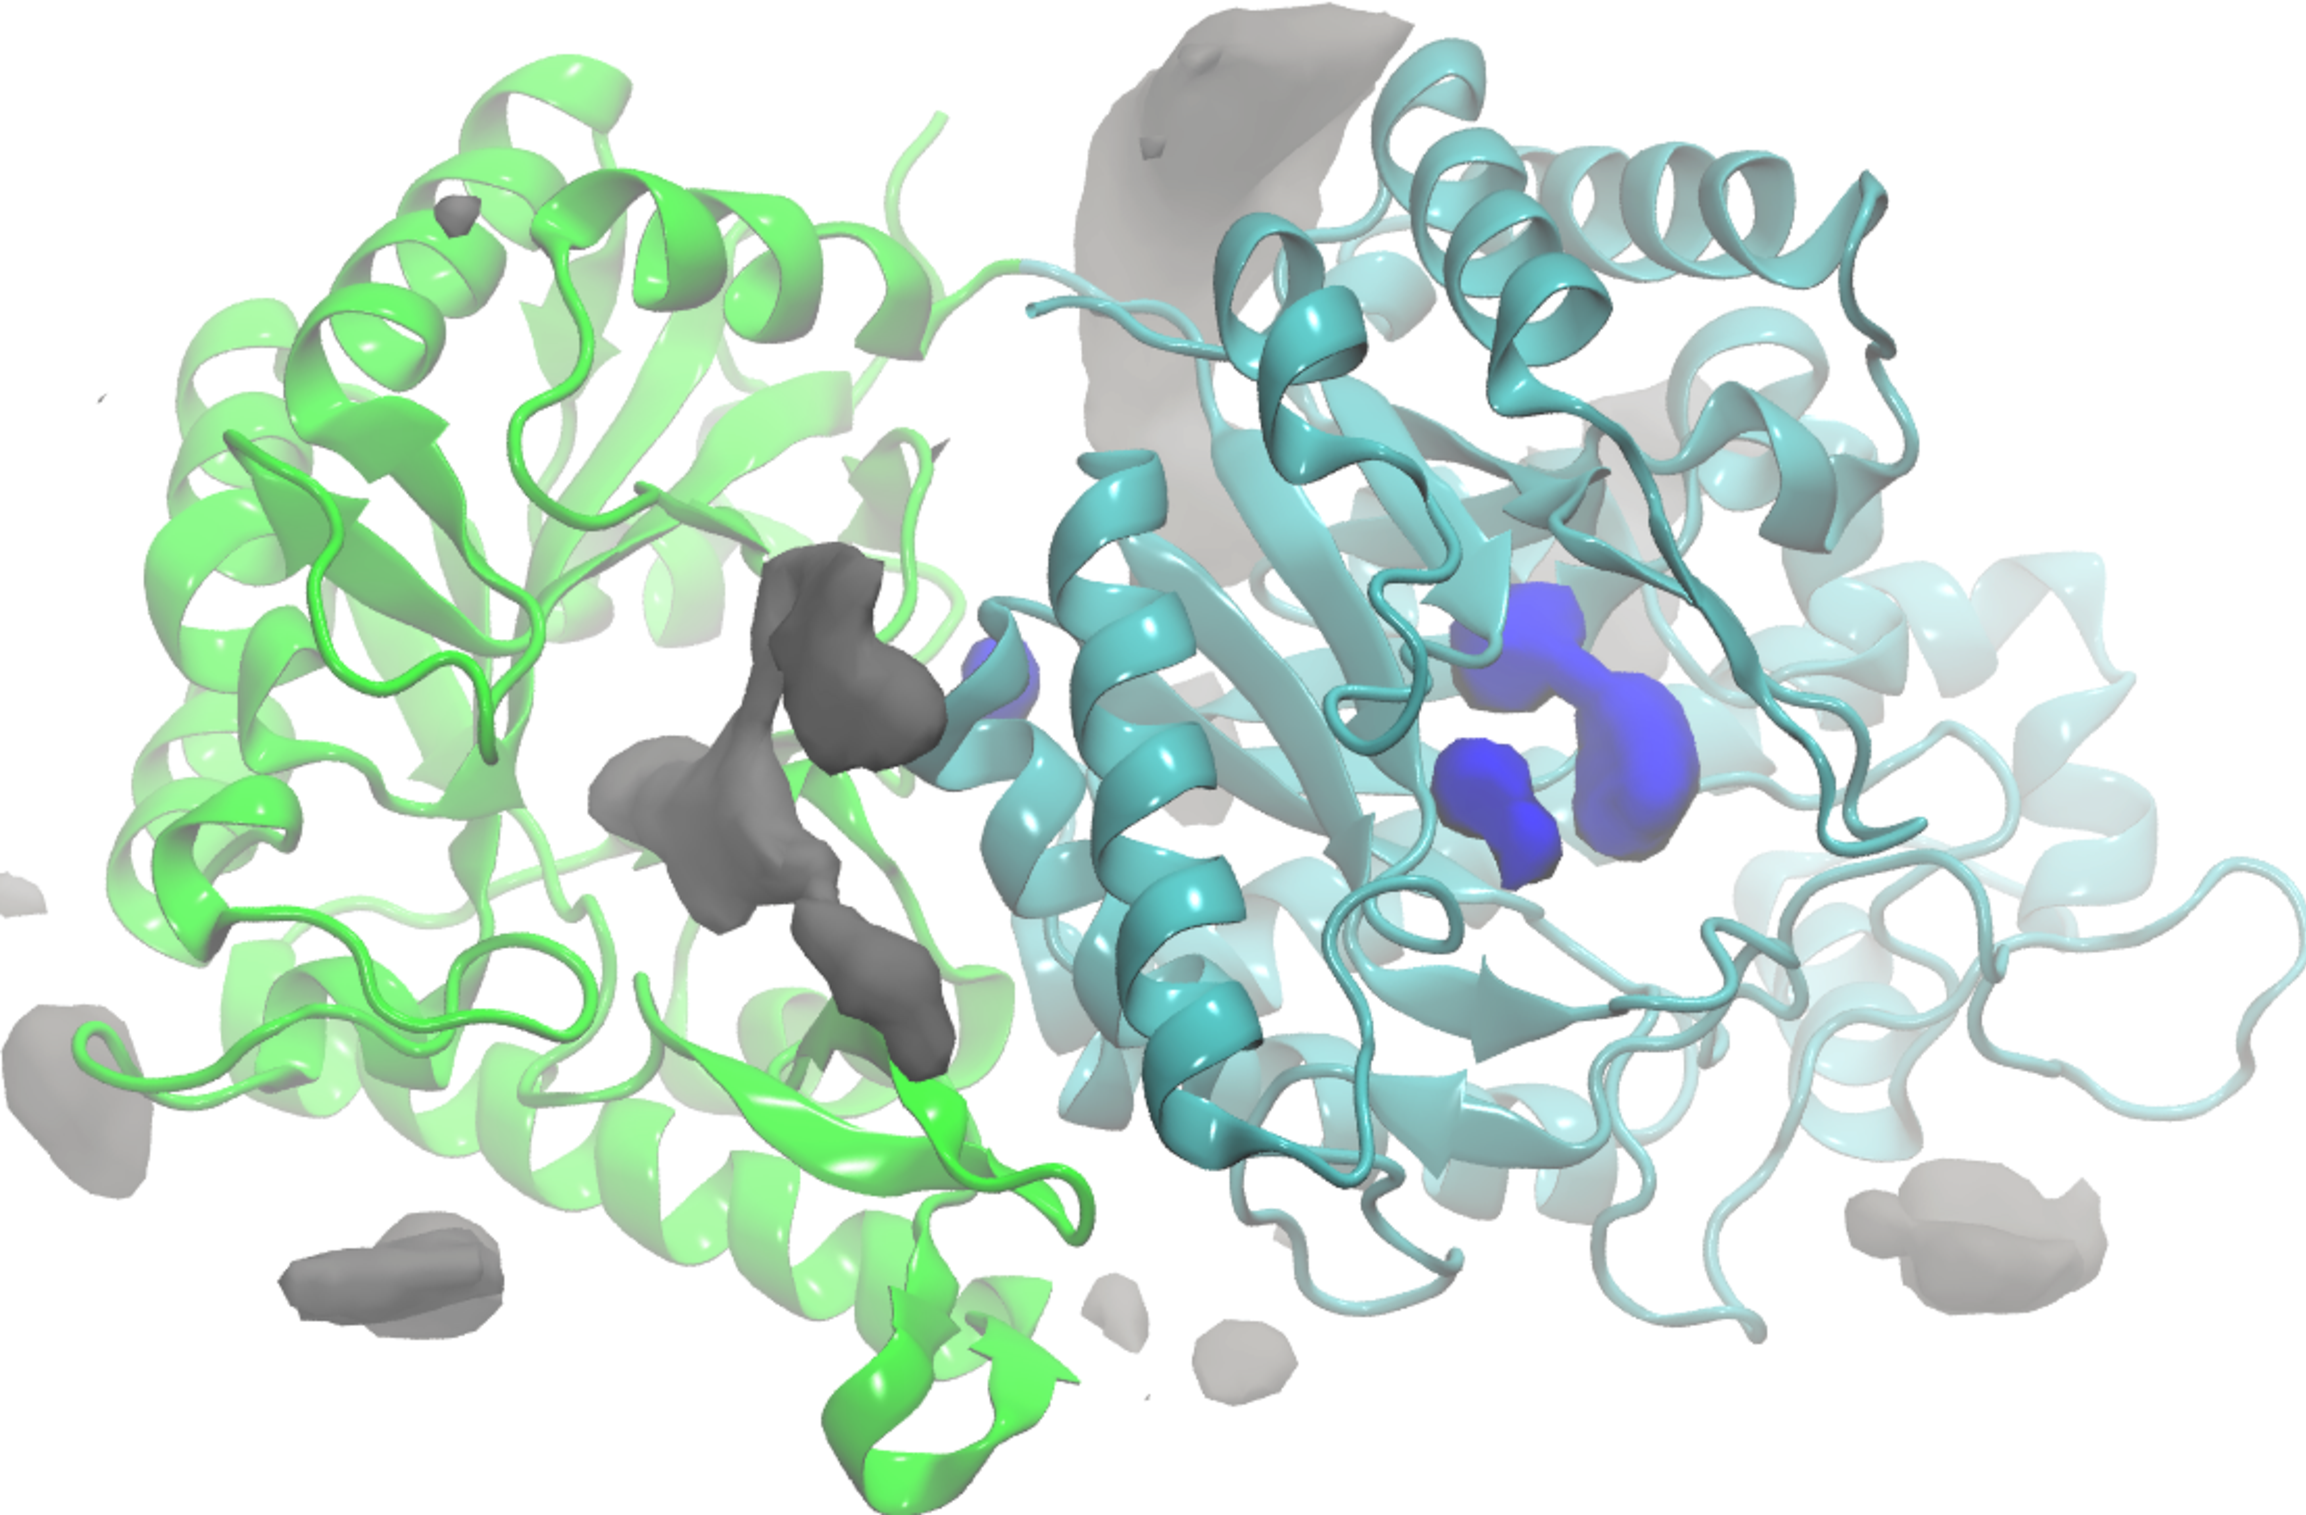
\includegraphics[width=6.25in]{figures/results4/pgab_glucosamine_salt_densities.pdf}
\caption[Ionic distribution]{Spatial probability distribution of sodium (blue) and chloride (grey) ions depicted at an isovalue of 0.005. The protein is depicted in a cartoon representation, with N- and C-terminal domains colored in green and cyan, respectively.}
\label{fig:salt_density_distribution}
\end{figure}

\begin{figure}[htbp]
\centering
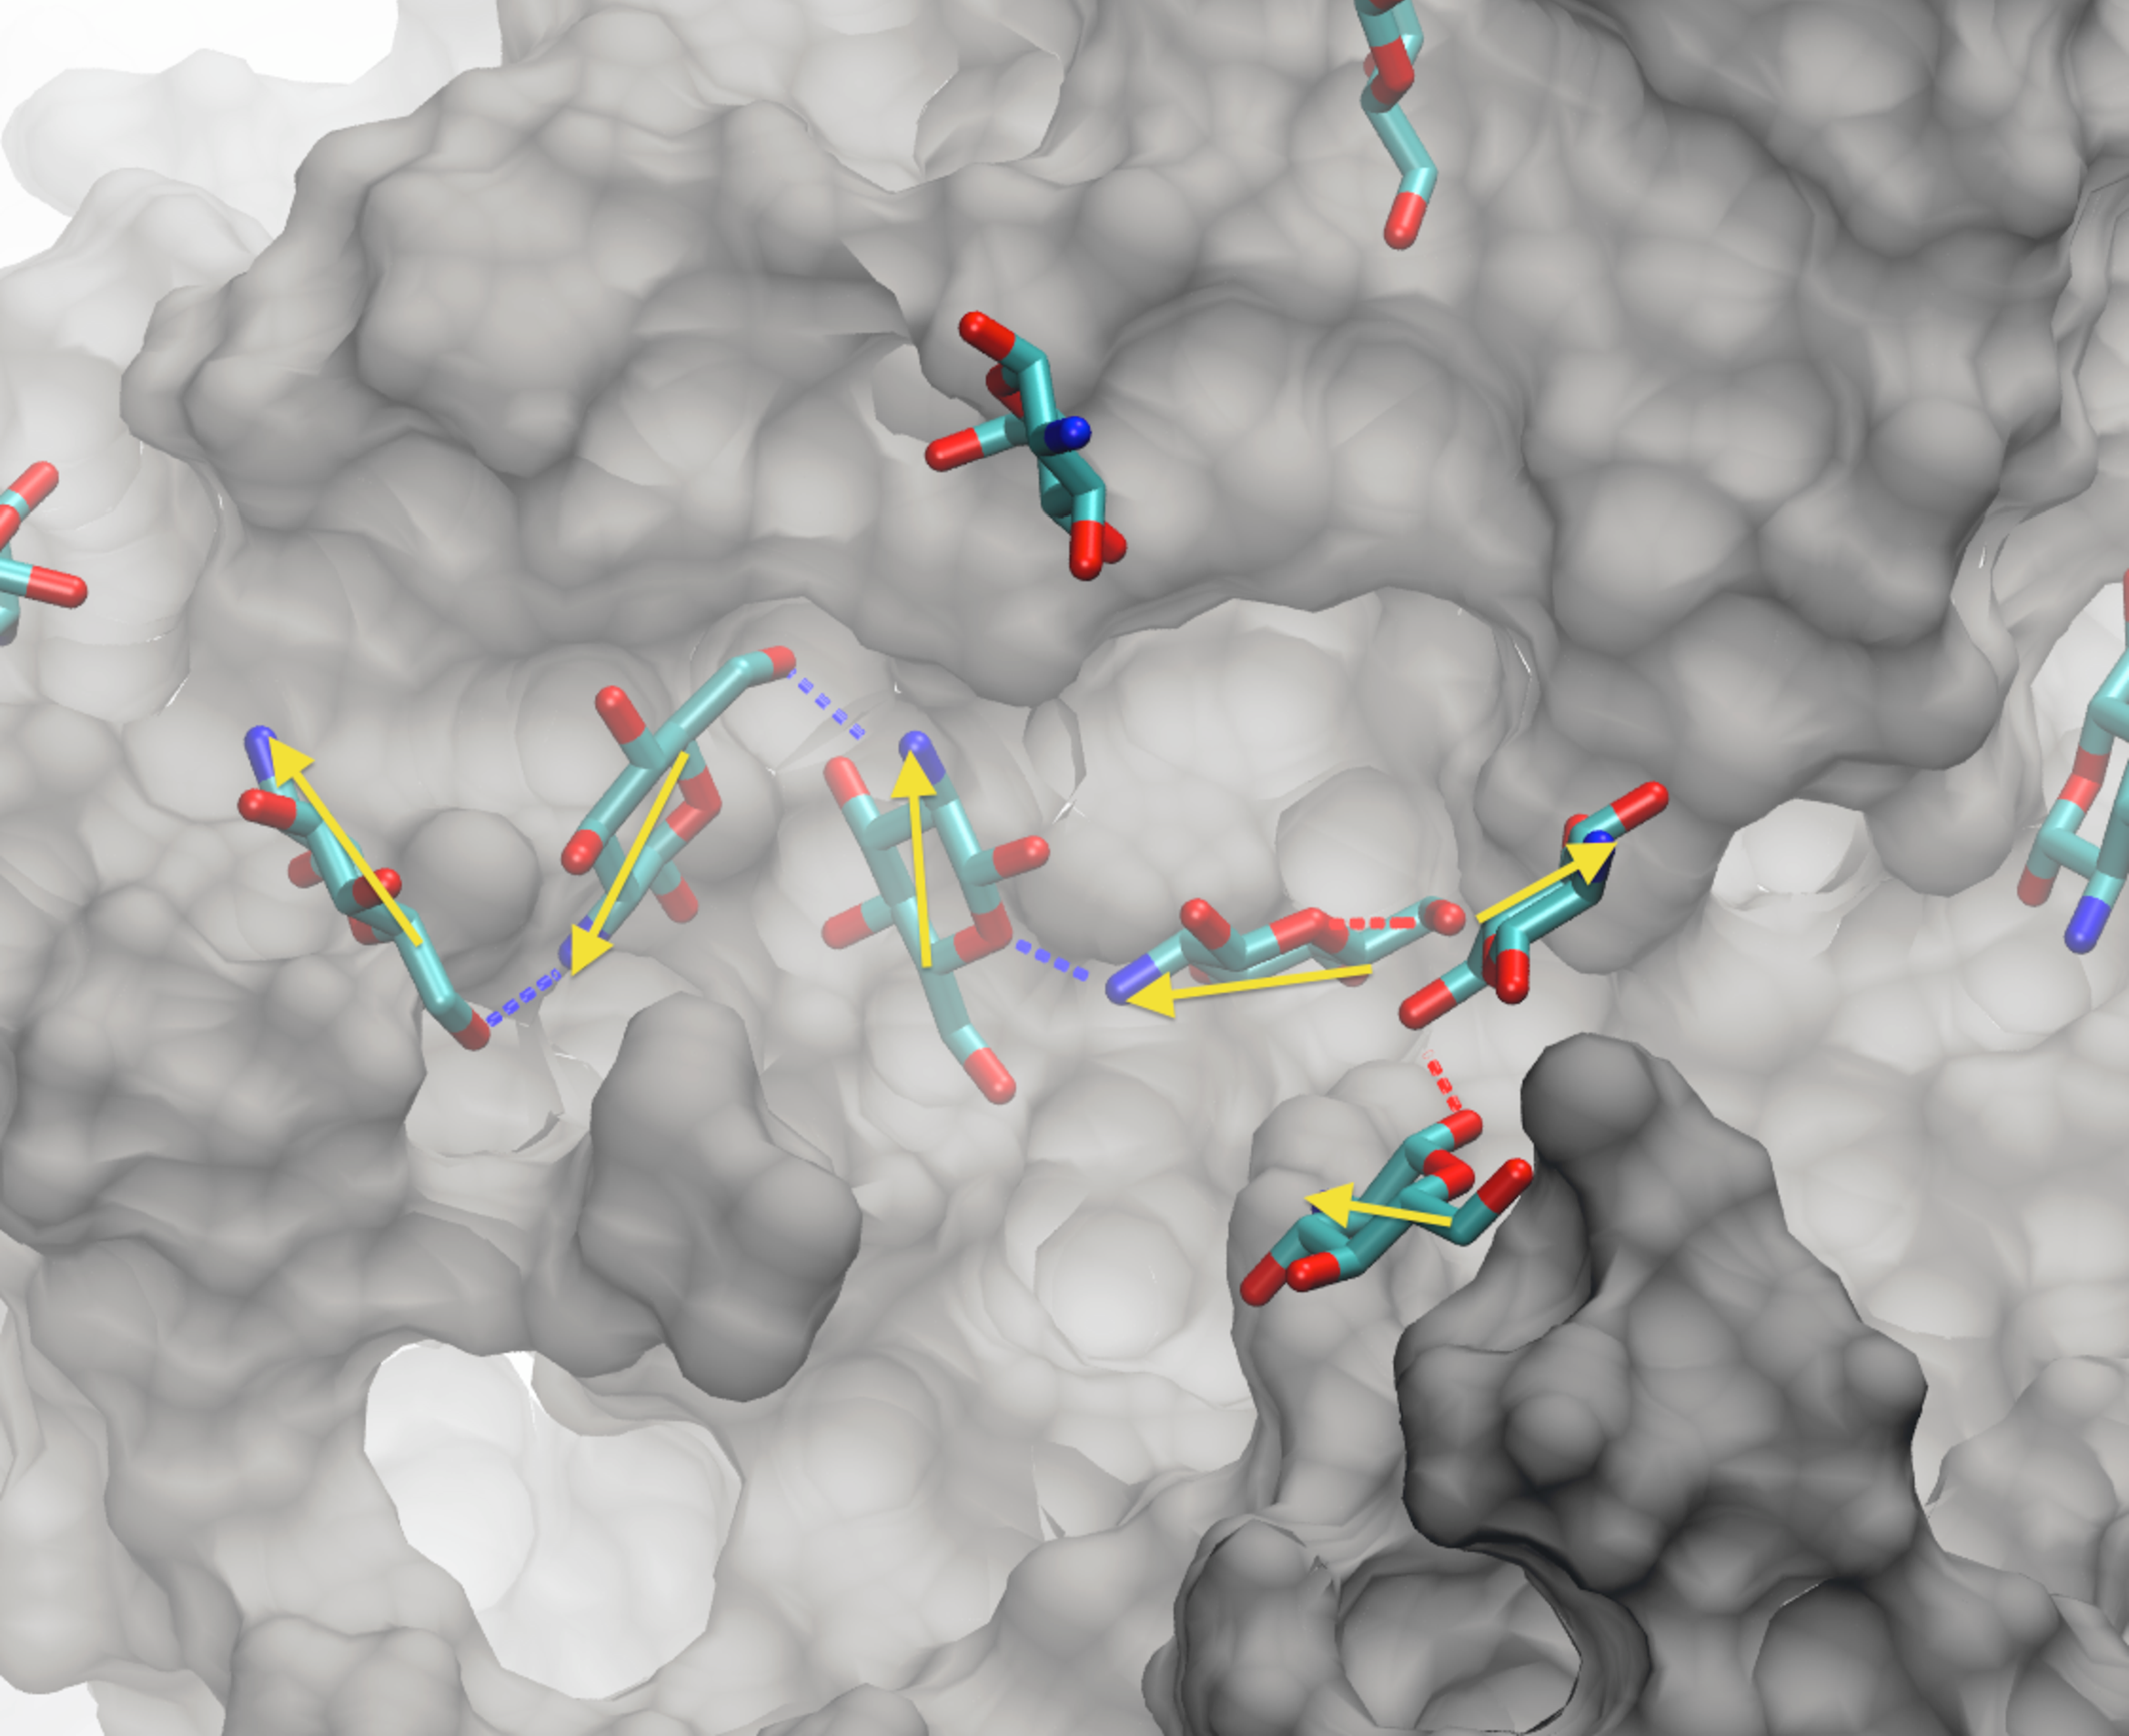
\includegraphics[width=6.25in]{figures/results4/glucosamine_binding_direction_suggestive.pdf}
\caption[Polymer directionality]{A linear chain of hydrogen-bonded \glucosamine\ molecules in the putative carbohydrate-binding groove of the C-terminal domain.  The yellow arrows are drawn as a guide to highlight a putative chain directionality.}
\label{fig:directionality}
\end{figure}

\begin{singlespace}
\addcontentsline{toc}{section}{Bibliography}
\bibliographystyle{elsart-num}
\bibliography{/Users/grace/github/thesis/document/results4/results4}
\end{singlespace}





